\documentclass{beamer}
\usepackage{graphicx}
\usepackage{bm}
\usepackage{xcolor}
\usepackage[ruled]{algorithm}
\usepackage{algorithmicx}
\usepackage[noend]{algpseudocode}
\usepackage{amsmath}
\usepackage{amssymb}

\begin{document}
\beamertemplatenavigationsymbolsempty

\title{Temporal Smoothing in 2D Human Pose Estimation for Bouldering}

\author{André Oskar Andersen
\newline \small \texttt{wpr684}}

\institute{Institution of Computer Science, University of Copenhagen}

\date{2023}

\newcommand\unfootnote[1]{%
  \begingroup
  \renewcommand\thefootnote{}\footnote{#1}%
  \addtocounter{footnote}{-1}%
  \endgroup
}

\frame{\titlepage}

\begin{frame}
    \frametitle{Introduction}
    \begin{minipage}{0.5\textwidth}
        \begin{itemize}
            \item<1-> Increased usage of video analysis in sports.
            \begin{itemize}
                \item Help referee
                \item Improve techniques
            \end{itemize}
        \end{itemize}
    \end{minipage} \hfill
    \begin{minipage}{0.45\textwidth}
        \begin{figure}
            \center
            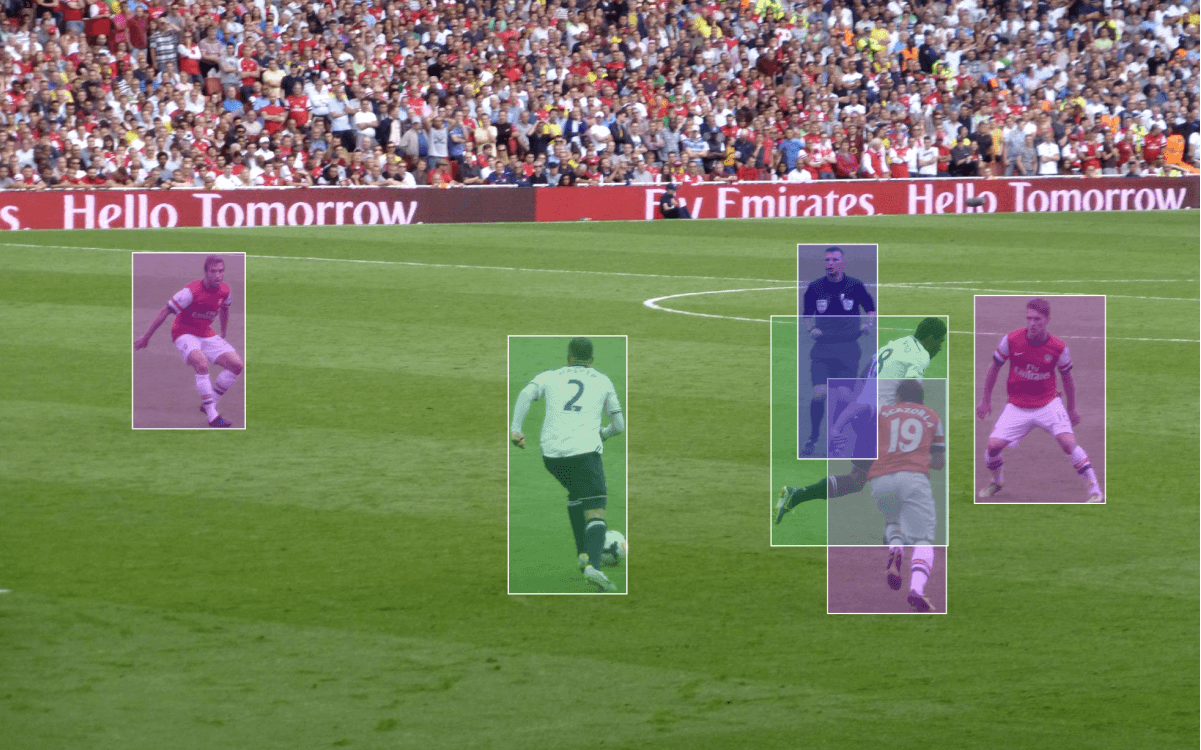
\includegraphics[width = \textwidth]{./entities/soccer_cv.png}
        \end{figure}
    \end{minipage}
    \unfootnote{\tiny \url{https://www.superannotate.com/blog/computer-vision-in-sports}}
\end{frame}

\begin{frame}
    \frametitle{Introduction}
    \begin{minipage}{0.5\textwidth}
        \begin{itemize}
            \item<1-> Increased usage of video analysis in sports.
            \item<1-> Often requires the position of the players.
            \begin{itemize}
                \item Already developed for popular sports.
                \item Missing for the less popular sports.
            \end{itemize}
        \end{itemize}
    \end{minipage} \hfill
    \begin{minipage}{0.45\textwidth}
        \begin{figure}
            \center
            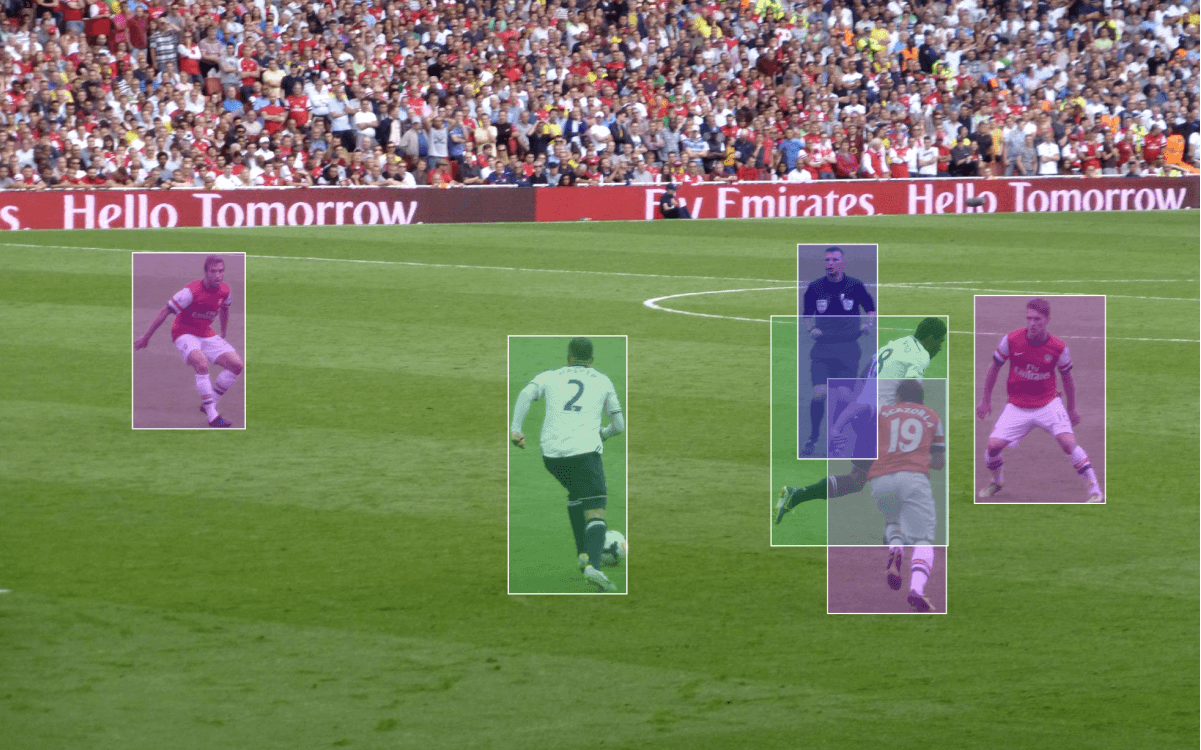
\includegraphics[width = \textwidth]{./entities/soccer_cv.png}
        \end{figure}
    \end{minipage}
    \unfootnote{\tiny \url{https://www.superannotate.com/blog/computer-vision-in-sports}}
\end{frame}

\begin{frame}
    \frametitle{Introduction}
    \begin{minipage}{0.5\textwidth}
        \begin{itemize}
            \item<1-> Increased usage of video analysis in sports.
            \item<1-> Often requires the position of the players.
            \item<1-> Problems with the data
            \begin{itemize}
                \item Methods require large quantities
                \item Unusual poses/movements
            \end{itemize}
        \end{itemize}
    \end{minipage} \hfill
    \begin{minipage}{0.45\textwidth}
        \begin{figure}
            \center
            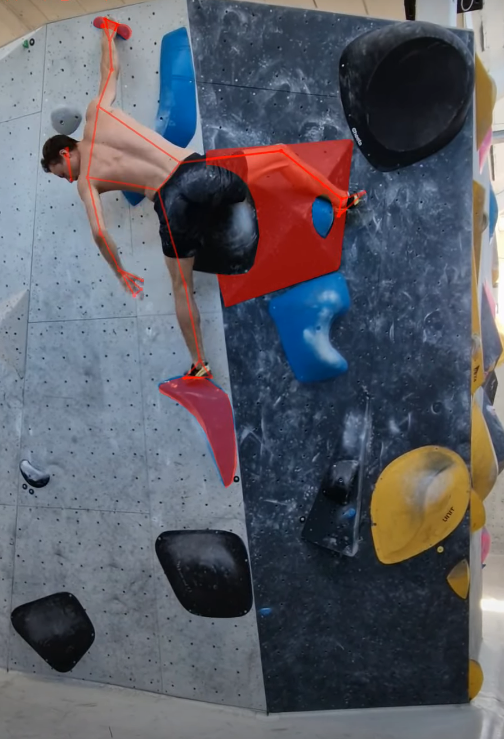
\includegraphics[width = \textwidth]{./entities/ClimbAlong_cv.PNG}
        \end{figure}
    \end{minipage}
    \unfootnote{\tiny \url{https://climbalong.com/lab}}
\end{frame}

\begin{frame}
    \frametitle{Introduction}
    \begin{minipage}{0.5\textwidth}
        \begin{itemize}
            \item<1-> Increased usage of video analysis in sports.
            \item<1-> Often requires the position of the players.
            \item<1-> Problems with the data
            \item<1-> ClimbAlong at NorthTech ApS
            \begin{itemize}
                \item<1-> Frame-idependent pose-detector for bouldering 
                \item<2-> Proposition: Incorporate temporal information
                % TODO: tilføj nogle frames?
            \end{itemize}
        \end{itemize}
    \end{minipage} \hfill
    \begin{minipage}{0.45\textwidth}
        \begin{figure}
            \center
            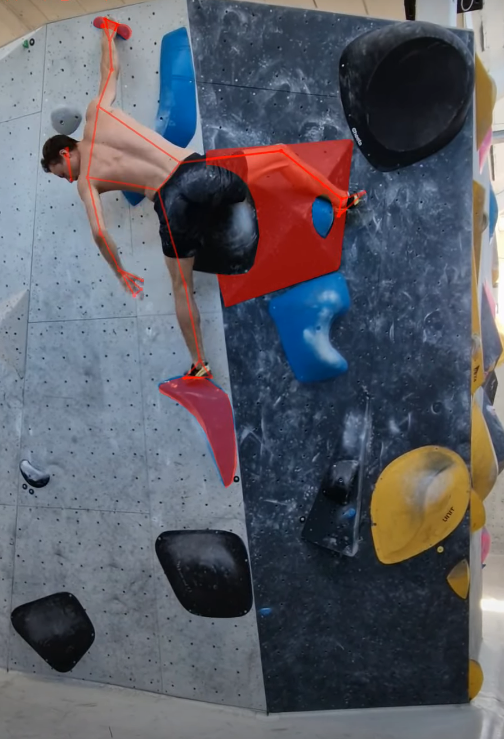
\includegraphics[width = \textwidth]{./entities/ClimbAlong_cv.PNG}
        \end{figure}
    \end{minipage}
    \unfootnote{\tiny \url{https://climbalong.com/lab}}
\end{frame}

\begin{frame}
    \frametitle{Introduction}
    \begin{itemize}
        \item<1-> Aim: extend the ClimbAlong pose-detector to use temporal information.
    \end{itemize}
\end{frame}

\begin{frame}
    \frametitle{The Data}
    \begin{minipage}{0.5\textwidth}
        ClimbAlong
        \begin{itemize}
            \item Fully annoated videos of climbers
            \item<2-> Problem: very small dataset
            \begin{itemize}
                \item BRACE
                \item Penn Action
            \end{itemize}
            % TODO: tilføj visualizations
        \end{itemize}
    \end{minipage} \hfill
    \begin{minipage}{0.45\textwidth}
        \begin{figure}
            \center
            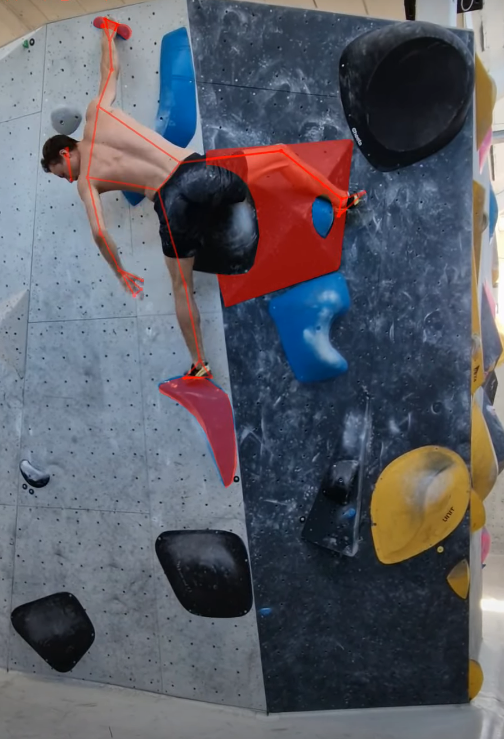
\includegraphics[width = \textwidth]{./entities/ClimbAlong_cv.PNG}
        \end{figure}
    \end{minipage}
    \unfootnote{\tiny \url{https://climbalong.com/lab}}
\end{frame}

\begin{frame}
    \frametitle{The Data}
    \begin{minipage}{0.5\textwidth}
        ClimbAlong
        \begin{itemize}
            \item Fully annoated videos of climbers
            \item Problem: Very small dataset
            \item Solution: pretrain on related datasets and finetune on ClimbAlong
            \begin{itemize}
                \item BRACE
                \item Penn Action
            \end{itemize}
            % TODO: tilføj visualizations
        \end{itemize}
    \end{minipage} \hfill
    \begin{minipage}{0.45\textwidth}
        \begin{figure}
            \center
            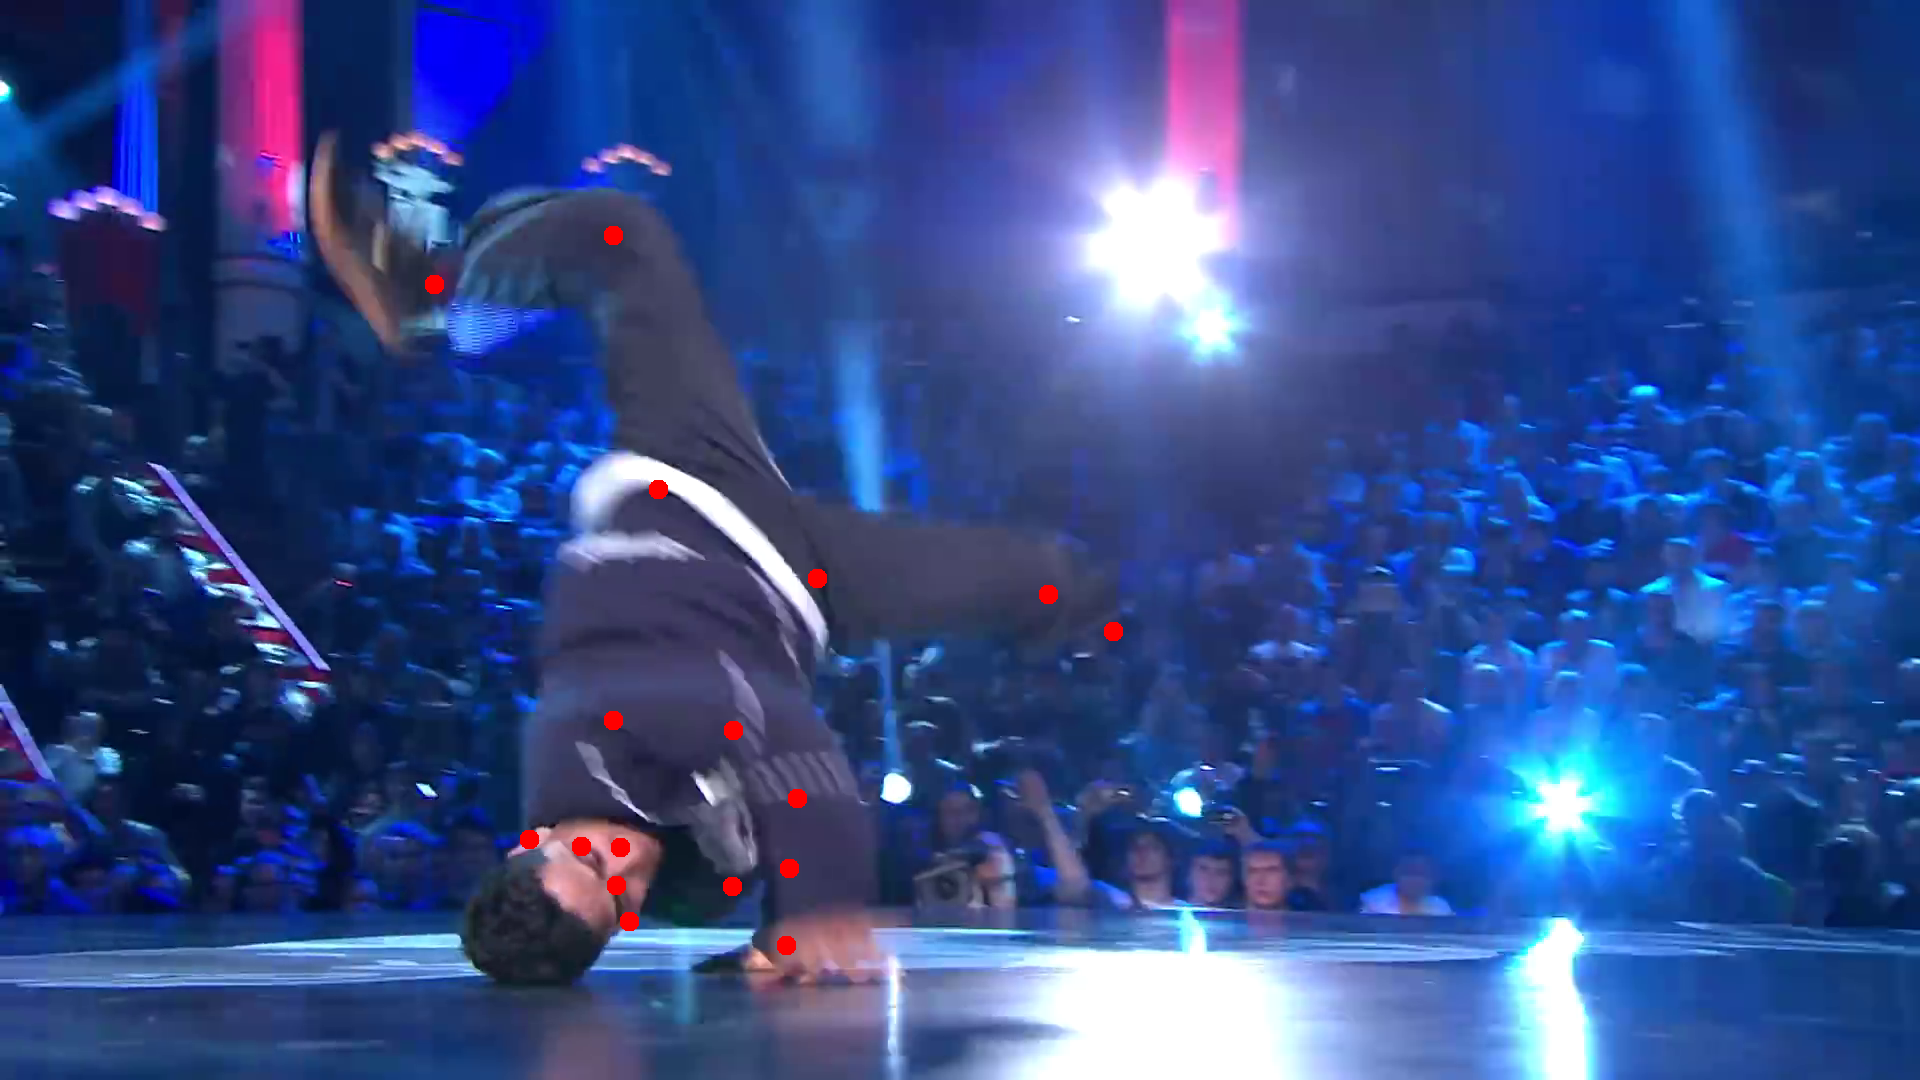
\includegraphics[width = \textwidth]{../report/entities/BRACE_1152.png}
            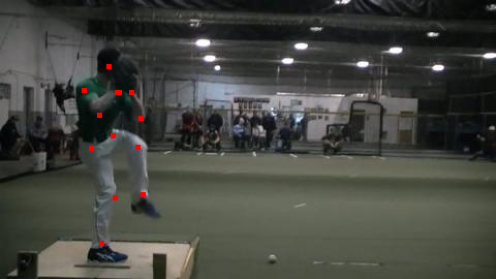
\includegraphics[width = \textwidth]{../report/entities/PA_64.png}
        \end{figure}
    \end{minipage}
\end{frame}

\begin{frame}
    \frametitle{The Models}
    Generally, three approaches
    \begin{enumerate}
        \item Convolutional layer
        \item Recurrent neural network
        \item Transformer
    \end{enumerate}
\end{frame}

\begin{frame}
    \frametitle{The Models}
    3DConv
    \begin{itemize}
        \item<1-> 3-dimensional conv. layer + ReLU
    \end{itemize}
    \begin{figure}
        \centering
        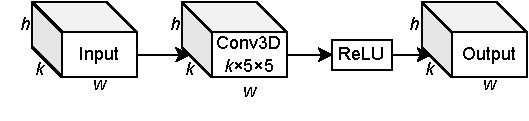
\includegraphics[width = 0.8\textwidth]{../report/entities/baseline.pdf}
    \end{figure}
\end{frame}

\begin{frame}
    \frametitle{The Models}
    bi-ConvLSTM Model S
    \begin{itemize}
        \item<1-> Adaptation of Unipose-LSTM by Artacho and Savakis
        \item<1-> Bidirectional convolutional LSTM + conv. layers and ReLU
        \item<1-> Processing directions summed together
    \end{itemize}
    \begin{figure}
        \centering
        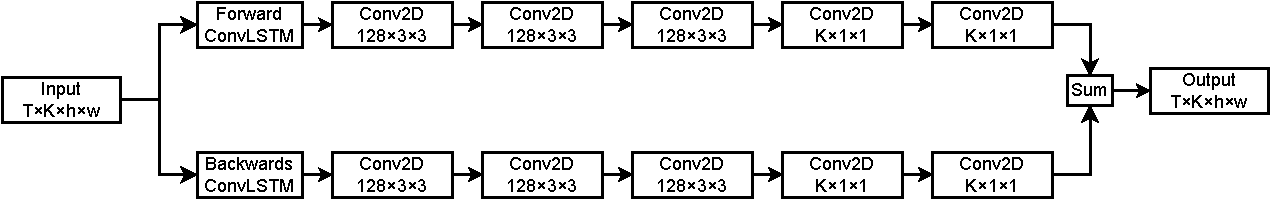
\includegraphics[width = \textwidth]{../report/entities/bi_conv_lstm.pdf}
    \end{figure}
    \unfootnote{\tiny \url{https://openaccess.thecvf.com/content_CVPR_2020/papers/Artacho_UniPose_Unified_Human_Pose_Estimation_in_Single_Images_and_Videos_CVPR_2020_paper.pdf}}
\end{frame}

\begin{frame}
    \frametitle{The Models}
    bi-ConvLSTM Model C
    \begin{itemize}
        \item<1-> Problem: Prioritization of processing direction
        \item<1-> Solution: Using convolution
    \end{itemize}
    \begin{figure}
        \centering
        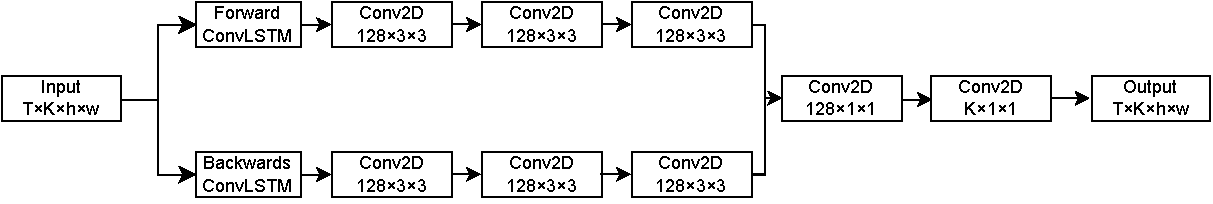
\includegraphics[width = \textwidth]{../report/entities/unipose2.pdf}
    \end{figure}
\end{frame}

\begin{frame}
    \frametitle{The Models}
    DeciWatch by Zeng \textit{Et al}.
    \begin{itemize}
        \item<1-> Transformer-based
        \item<1-> Samples every $n$th frame
        \item<1-> DenoiseNet + RecoverNet
    \end{itemize}
    \begin{figure}
        \centering
        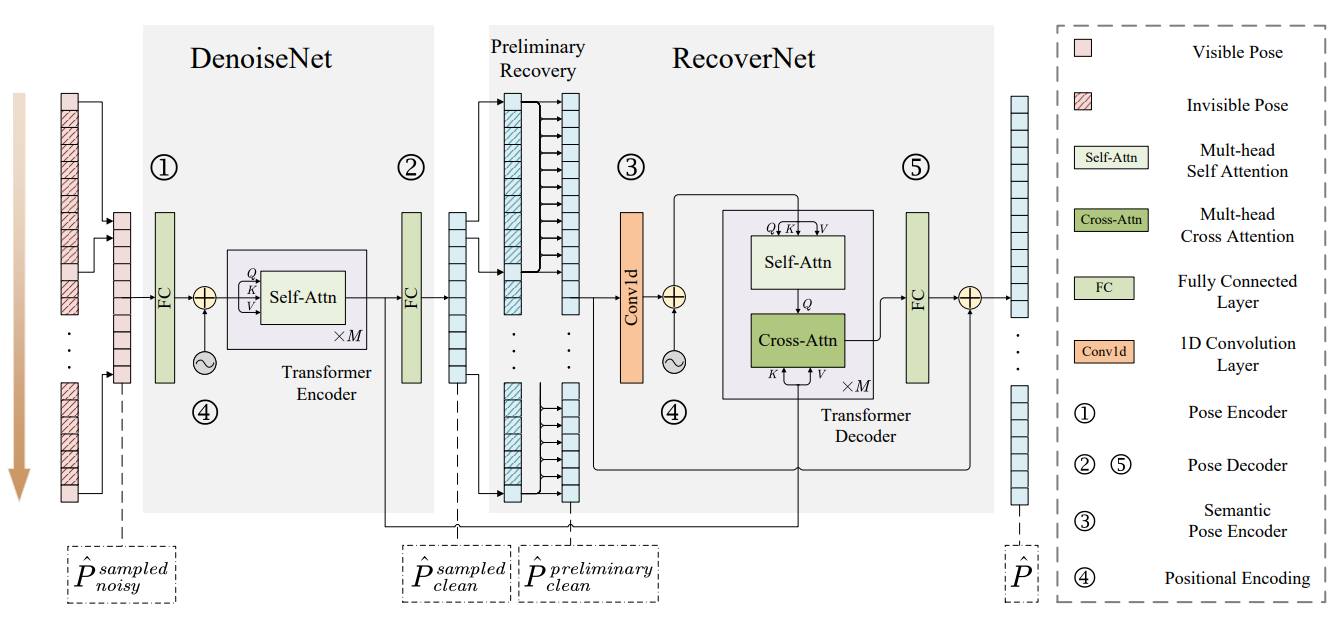
\includegraphics[width = \textwidth]{../report/entities/deciwatch.PNG}
    \end{figure}
    \unfootnote{\tiny \url{https://arxiv.org/pdf/2203.08713.pdf}}
\end{frame}

\begin{frame}
    \frametitle{Pretraining}
    Procedure
    \begin{itemize}
        \item<1-> Not training already-developed pose-detector
        \begin{itemize}
            \item Different input images
        \end{itemize}
        \item<2-> Instead, simulate pose-detector output by shifting keypoints
    \end{itemize}
\end{frame}

\begin{frame}
    \frametitle{Pretraining}
    Finding optimal setting of models
    \begin{itemize}
        \item<1-> Three experiments
        \begin{enumerate}
            \item<1-> Various smearing standard deviations
            \item<2-> Fixed smearing standard deviation
            \item<3-> Smearing standard deviations + decreased frame rate
        \end{enumerate}
        \item<4-> Two different shifting-scalars
    \end{itemize}
    \begin{figure}
        \centering
        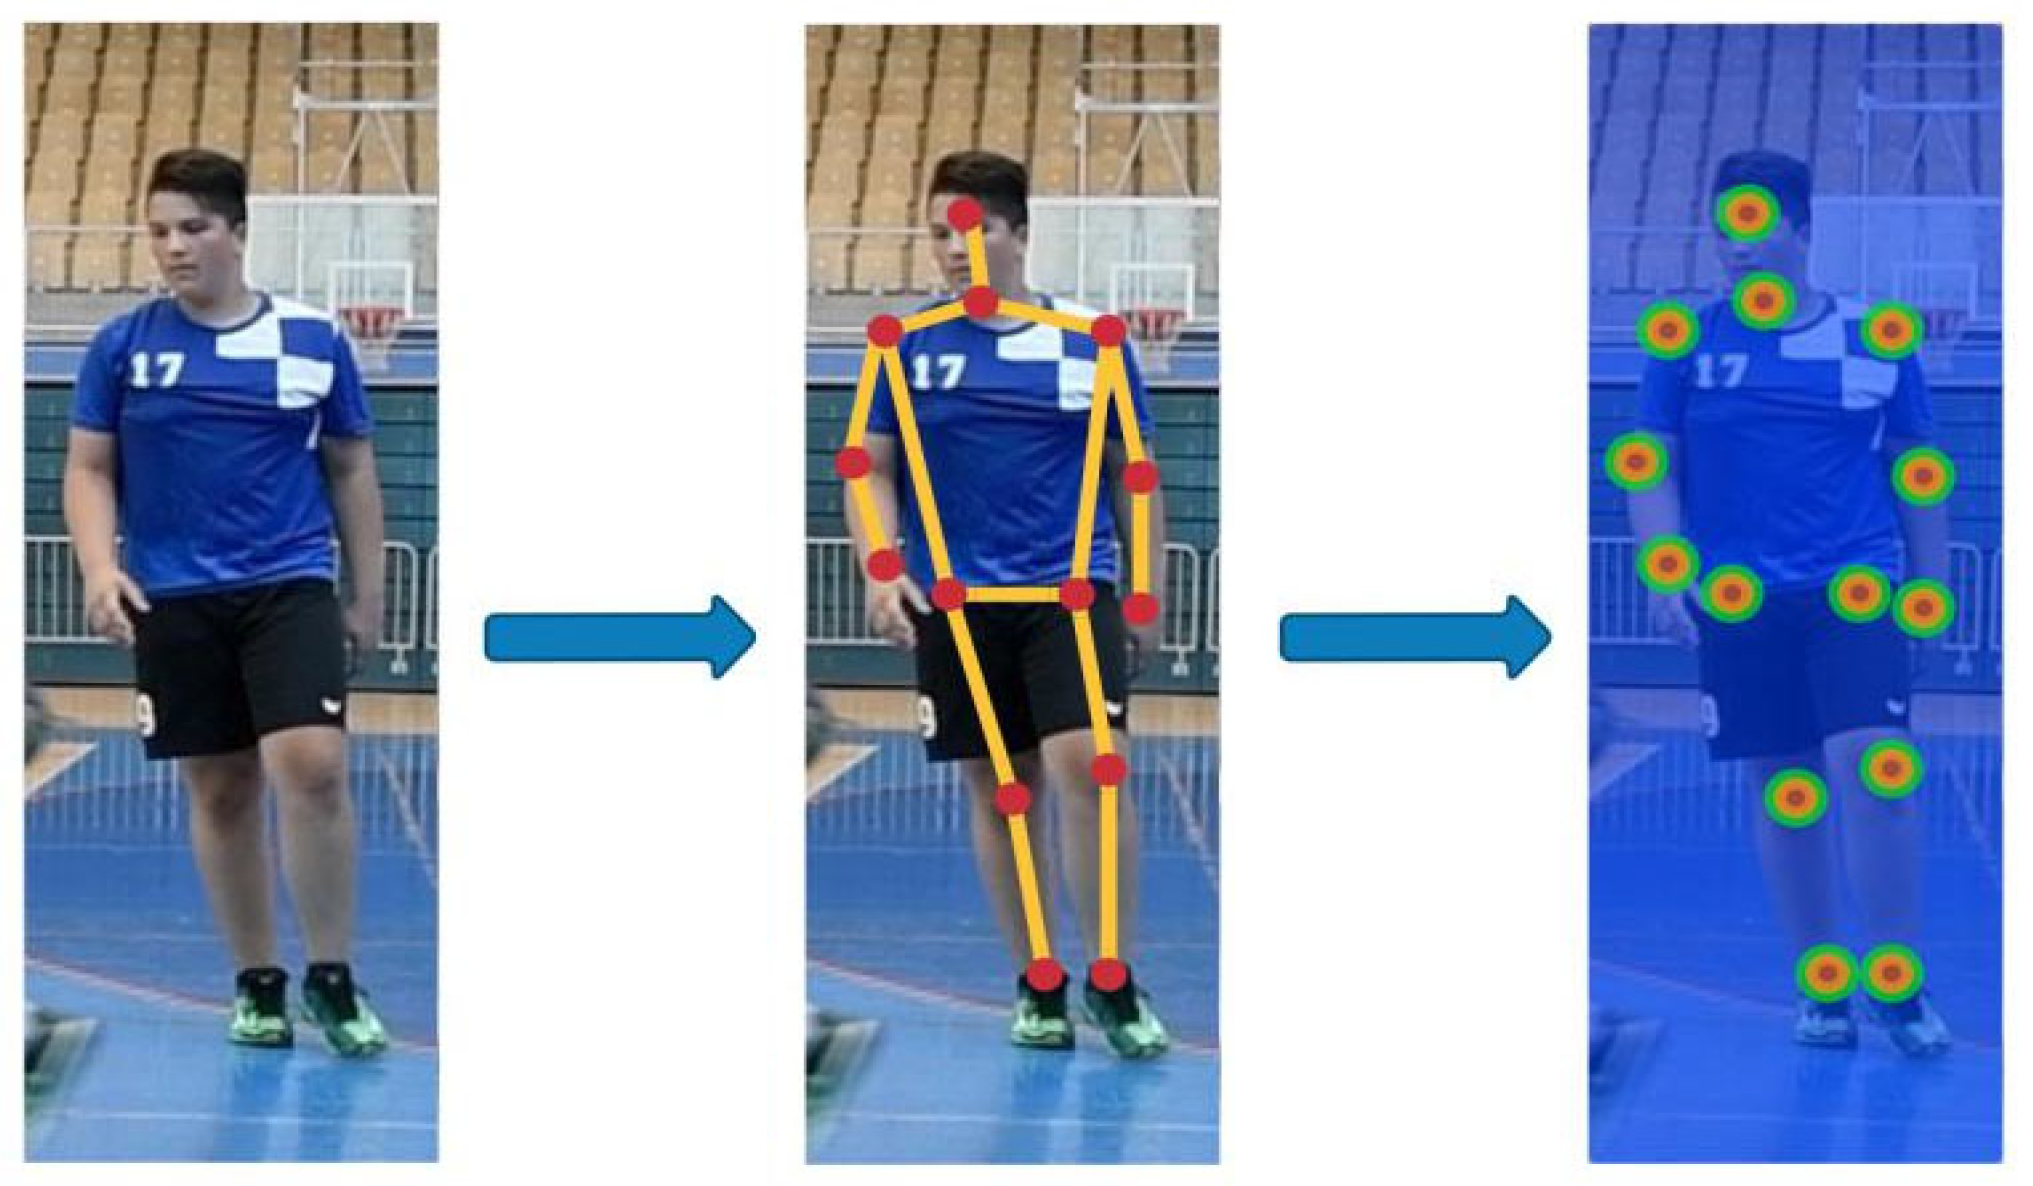
\includegraphics[width = 0.7 \textwidth]{./entities/heatmaps.png}
    \end{figure}
    \unfootnote{\tiny \url{https://www.mdpi.com/2313-433X/8/11/308}}
\end{frame}

\begin{frame}
    \frametitle{Finetuning}
    \begin{itemize}
        \item<1-> Using all of the developed models with pose-detector
        \item<1-> Freezing pose-detector
        \begin{enumerate}
            \item Quicker fitting
            \item Greater understanding of results  
        \end{enumerate}
    \end{itemize}
\end{frame}

\begin{frame}
    \frametitle{Finetuning}
    Test results
    \begin{itemize}
        \item Shifting-scalar: only minor effect
    \end{itemize}
    \begin{table}[htbp]
        \scalebox{0.7}{
            \begin{tabular}{c||ccc|ccc|ccc}
                \hline
                Accuracy metric & \multicolumn{3}{c}{PCK@0.05} & \multicolumn{3}{c}{PCK@0.1} & \multicolumn{3}{c}{PCK@0.2} \\
                \hline
                Experiment & 1.1 & 1.2 & 1.3 & 1.1 & 1.2 & 1.3 & 1.1 & 1.2 & 1.3 \\
                \hline
                \hline
                Identity function & 19.4 & 19.4 & 19.4 & 66.1 & 66.1 & 66.1 & 85.2 & 85.2 & 85.2 \\
                3DConv & \textcolor{green}{49.7} & \textcolor{green}{52.3} & \textcolor{green}{53.1} & \textcolor{green}{95.7} & \textcolor{green}{95.7} & \textcolor{black}{95.8} & \textcolor{black}{99.2} & \textcolor{black}{99.3} & \textcolor{green}{99.3} \\
                DeciWatch & \textcolor{green}{76.6} & \textcolor{green}{76.7} & \textcolor{green}{68.1} & \textcolor{green}{94.4} & \textcolor{green}{94.3} & \textcolor{green}{87.3} & \textcolor{black}{99.2} & \textcolor{black}{99.2} & \textcolor{green}{96.1} \\
                bi-ConvLSTM - Model S & \textcolor{red}{37.8} & \textcolor{red}{34.9} & \textcolor{green}{39.0} & \textcolor{red}{91.8} & \textcolor{black}{92.1} & \textcolor{green}{92.2} & \textcolor{black}{99.4} & \textcolor{green}{99.7} & \textcolor{red}{99.2} \\
                bi-ConvLSTM - Model C & \textcolor{red}{35.9} & \textcolor{red}{39.0} & \textcolor{green}{38.5} & \textcolor{green}{93.1} & \textcolor{green}{93.6} & \textcolor{black}{92.6} & \textcolor{green}{99.8} & \textcolor{green}{99.7} & \textcolor{green}{99.7} \\
                \hline
            \end{tabular}
        }
    \end{table}
    
    \begin{table}[htbp]
        \scalebox{0.7}{
            \begin{tabular}{c||ccc|ccc|ccc}
                \hline
                Accuracy metric & \multicolumn{3}{c}{PCK@0.05} & \multicolumn{3}{c}{PCK@0.1} & \multicolumn{3}{c}{PCK@0.2} \\
                \hline
                Experiment & 2.1 & 2.2 & 2.3 & 2.1 & 2.2 & 2.3 & 2.1 & 2.2 & 2.3 \\
                \hline
                \hline
                Identity function & 19.4 & 19.4 & 19.4 & 66.1 & 66.1 & 66.1 & 85.2 & 85.2 & 85.2 \\
                3DConv & \textcolor{red}{46.5} & \textcolor{red}{51.6} & \textcolor{red}{47.3} & \textcolor{red}{95.5} & \textcolor{red}{95.5} & \textcolor{black}{95.8} & \textcolor{black}{99.2} & \textcolor{black}{99.3} & \textcolor{red}{99.2} \\
                DeciWatch & \textcolor{red}{76.0} & \textcolor{red}{75.9} & \textcolor{red}{36.8} & \textcolor{red}{94.2} & \textcolor{red}{94.2} & \textcolor{red}{74.9} & \textcolor{black}{99.2} & \textcolor{black}{99.2} & \textcolor{red}{92.8} \\
                bi-ConvLSTM - Model S & \textcolor{green}{38.8} & \textcolor{green}{37.4} & \textcolor{red}{35.9} & \textcolor{green}{92.7} & \textcolor{black}{92.1} & \textcolor{red}{91.2} & \textcolor{black}{99.4} & \textcolor{red}{99.5} & \textcolor{green}{99.3} \\
                bi-ConvLSTM - Model C & \textcolor{green}{39.2} & \textcolor{green}{39.5} & \textcolor{red}{37.1} & \textcolor{red}{92.5} & \textcolor{red}{92.9} & \textcolor{black}{92.6} & \textcolor{red}{99.6} & \textcolor{red}{99.3} & \textcolor{red}{99.6} \\
                \hline
            \end{tabular}
        }
    \end{table}
\end{frame}

\begin{frame}
    \frametitle{Finetuning}
    Test results
    \begin{itemize}
        \item 3DConv: translation + scaling vs only translation
    \end{itemize}
    \begin{table}[htbp]
        \scalebox{0.7}{
            \begin{tabular}{c||ccc|ccc|ccc}
                \hline
                Accuracy metric & \multicolumn{3}{c}{PCK@0.05} & \multicolumn{3}{c}{PCK@0.1} & \multicolumn{3}{c}{PCK@0.2} \\
                \hline
                Experiment & 1.1 & 1.2 & 1.3 & 1.1 & 1.2 & 1.3 & 1.1 & 1.2 & 1.3 \\
                \hline
                \hline
                Identity function & 19.4 & 19.4 & 19.4 & 66.1 & 66.1 & 66.1 & 85.2 & 85.2 & 85.2 \\
                3DConv & \textcolor{red}{49.7} & \textcolor{green}{52.3} & 53.1 & \textcolor{yellow}{95.7} & \textcolor{yellow}{95.7} & 95.8 & \textcolor{red}{99.2} & \textcolor{green}{99.3} & 99.3 \\
                DeciWatch & 76.6 & 76.7 & 68.1 & 94.4 & 94.3 & 87.3 & 99.2 & 99.2 & 96.1 \\
                bi-ConvLSTM - Model S & 37.8 & 34.9 & 39.0 & 91.8 & 92.1 & 92.2 & 99.4 & 99.7 & 99.2 \\
                bi-ConvLSTM - Model C & 35.9 & 39.0 & 38.5 & 93.1 & 93.6 & 92.6 & 99.8 & 99.7 & 99.7 \\
                \hline
            \end{tabular}
        }
    \end{table}
    
    \begin{table}[htbp]
        \scalebox{0.7}{
            \begin{tabular}{c||ccc|ccc|ccc}
                \hline
                Accuracy metric & \multicolumn{3}{c}{PCK@0.05} & \multicolumn{3}{c}{PCK@0.1} & \multicolumn{3}{c}{PCK@0.2} \\
                \hline
                Experiment & 2.1 & 2.2 & 2.3 & 2.1 & 2.2 & 2.3 & 2.1 & 2.2 & 2.3 \\
                \hline
                \hline
                Identity function & 19.4 & 19.4 & 19.4 & 66.1 & 66.1 & 66.1 & 85.2 & 85.2 & 85.2 \\
                3DConv & \textcolor{red}{46.5} & \textcolor{green}{51.6} & 47.3 & \textcolor{yellow}{95.5} & \textcolor{yellow}{95.5} & 95.8 & \textcolor{red}{99.2} & \textcolor{green}{99.3} & 99.2 \\
                DeciWatch & 76.0 & 75.9 & 36.8 & 94.2 & 94.2 & 74.9 & 99.2 & 99.2 & 92.8 \\
                bi-ConvLSTM - Model S & 38.8 & 37.4 & 35.9 & 92.7 & 92.1 & 91.2 & 99.4 & 99.5 & 99.3 \\
                bi-ConvLSTM - Model C & 39.2 & 39.5 & 37.1 & 92.5 & 92.9 & 92.6 & 99.6 & 99.3 & 99.6 \\
                \hline
            \end{tabular}
        }
    \end{table}
\end{frame}

\begin{frame}
    \frametitle{Finetuning}
    Test results
    \begin{itemize}
        \item DeciWatch: effects of decreased frame rate
    \end{itemize}
    \begin{table}[htbp]
        \scalebox{0.7}{
            \begin{tabular}{c||ccc|ccc|ccc}
                \hline
                Accuracy metric & \multicolumn{3}{c}{PCK@0.05} & \multicolumn{3}{c}{PCK@0.1} & \multicolumn{3}{c}{PCK@0.2} \\
                \hline
                Experiment & 1.1 & 1.2 & 1.3 & 1.1 & 1.2 & 1.3 & 1.1 & 1.2 & 1.3 \\
                \hline
                \hline
                Identity function & 19.4 & 19.4 & 19.4 & 66.1 & 66.1 & 66.1 & 85.2 & 85.2 & 85.2 \\
                3DConv & 49.7 & 52.3 & 53.1 & 95.7 & 95.7 & 95.8 & 99.2 & 99.3 & 99.3 \\
                DeciWatch & \textcolor{green}{76.6} & 76.7 & \textcolor{red}{68.1} & \textcolor{green}{94.4} & 94.3 & \textcolor{red}{87.3} & \textcolor{green}{99.2} & 99.2 & \textcolor{red}{96.1} \\
                bi-ConvLSTM - Model S & 37.8 & 34.9 & 39.0 & 91.8 & 92.1 & 92.2 & 99.4 & 99.7 & 99.2 \\
                bi-ConvLSTM - Model C & 35.9 & 39.0 & 38.5 & 93.1 & 93.6 & 92.6 & 99.8 & 99.7 & 99.7 \\
                \hline
            \end{tabular}
        }
    \end{table}
    
    \begin{table}[htbp]
        \scalebox{0.7}{
            \begin{tabular}{c||ccc|ccc|ccc}
                \hline
                Accuracy metric & \multicolumn{3}{c}{PCK@0.05} & \multicolumn{3}{c}{PCK@0.1} & \multicolumn{3}{c}{PCK@0.2} \\
                \hline
                Experiment & 2.1 & 2.2 & 2.3 & 2.1 & 2.2 & 2.3 & 2.1 & 2.2 & 2.3 \\
                \hline
                \hline
                Identity function & 19.4 & 19.4 & 19.4 & 66.1 & 66.1 & 66.1 & 85.2 & 85.2 & 85.2 \\
                3DConv & 46.5 & 51.6 & 47.3 & 95.5 & 95.5 & 95.8 & 99.2 & 99.3 & 99.2 \\
                DeciWatch & \textcolor{green}{76.0} & 75.9 & \textcolor{red}{36.8} & \textcolor{green}{94.2} & 94.2 & \textcolor{red}{74.9} & \textcolor{green}{99.2} & 99.2 & \textcolor{red}{92.8} \\
                bi-ConvLSTM - Model S & 38.8 & 37.4 & 35.9 & 92.7 & 92.1 & 91.2 & 99.4 & 99.5 & 99.3 \\
                bi-ConvLSTM - Model C & 39.2 & 39.5 & 37.1 & 92.5 & 92.9 & 92.6 & 99.6 & 99.3 & 99.6 \\
                \hline
            \end{tabular}
        }
    \end{table}
\end{frame}

\begin{frame}
    \frametitle{Finetuning}
    Test results
    \begin{itemize}
        \item bi-ConvLSTM: Model S vs Model C
    \end{itemize}
    \begin{table}[htbp]
        \scalebox{0.7}{
            \begin{tabular}{c||ccc|ccc|ccc}
                \hline
                Accuracy metric & \multicolumn{3}{c}{PCK@0.05} & \multicolumn{3}{c}{PCK@0.1} & \multicolumn{3}{c}{PCK@0.2} \\
                \hline
                Experiment & 1.1 & 1.2 & 1.3 & 1.1 & 1.2 & 1.3 & 1.1 & 1.2 & 1.3 \\
                \hline
                \hline
                Identity function & 19.4 & 19.4 & 19.4 & 66.1 & 66.1 & 66.1 & 85.2 & 85.2 & 85.2 \\
                3DConv & 49.7 & 52.3 & 53.1 & 95.7 & 95.7 & 95.8 & 99.2 & 99.3 & 99.3 \\
                DeciWatch & 76.6 & 76.7 & 68.1 & 94.4 & 94.3 & 87.3 & 99.2 & 99.2 & 96.1 \\
                bi-ConvLSTM - Model S & \textcolor{green}{37.8} & \textcolor{red}{34.9} & \textcolor{green}{39.0} & \textcolor{red}{91.8} & \textcolor{red}{92.1} & \textcolor{red}{92.2} & \textcolor{red}{99.4} & \textcolor{yellow}{99.7} & \textcolor{red}{99.2} \\
                bi-ConvLSTM - Model C & \textcolor{red}{35.9} & \textcolor{green}{39.0} & \textcolor{red}{38.5} & \textcolor{green}{93.1} & \textcolor{green}{93.6} & \textcolor{green}{92.6} & \textcolor{green}{99.8} & \textcolor{yellow}{99.7} & \textcolor{green}{99.7} \\
                \hline
            \end{tabular}
        }
    \end{table}
    
    \begin{table}[htbp]
        \scalebox{0.7}{
            \begin{tabular}{c||ccc|ccc|ccc}
                \hline
                Accuracy metric & \multicolumn{3}{c}{PCK@0.05} & \multicolumn{3}{c}{PCK@0.1} & \multicolumn{3}{c}{PCK@0.2} \\
                \hline
                Experiment & 2.1 & 2.2 & 2.3 & 2.1 & 2.2 & 2.3 & 2.1 & 2.2 & 2.3 \\
                \hline
                \hline
                Identity function & 19.4 & 19.4 & 19.4 & 66.1 & 66.1 & 66.1 & 85.2 & 85.2 & 85.2 \\
                3DConv & 46.5 & 51.6 & 47.3 & 95.5 & 95.5 & 95.8 & 99.2 & 99.3 & 99.2 \\
                DeciWatch & 76.0 & 75.9 & 36.8 & 94.2 & 94.2 & 74.9 & 99.2 & 99.2 & 92.8 \\
                bi-ConvLSTM - Model S & \textcolor{red}{38.8} & \textcolor{red}{37.4} & \textcolor{red}{35.9} & \textcolor{green}{92.7} & \textcolor{red}{92.1} & \textcolor{red}{91.2} & \textcolor{red}{99.4} & \textcolor{green}{99.5} & \textcolor{red}{99.3} \\
                bi-ConvLSTM - Model C & \textcolor{green}{39.2} & \textcolor{green}{39.5} & \textcolor{green}{37.1} & \textcolor{red}{92.5} & \textcolor{green}{92.9} & \textcolor{green}{92.6} & \textcolor{green}{99.6} & \textcolor{red}{99.3} & \textcolor{green}{99.6} \\
                \hline
            \end{tabular}
        }
    \end{table}
\end{frame}

\begin{frame}
    \frametitle{Finetuning}
    Test results
    \begin{figure}
        \centering
        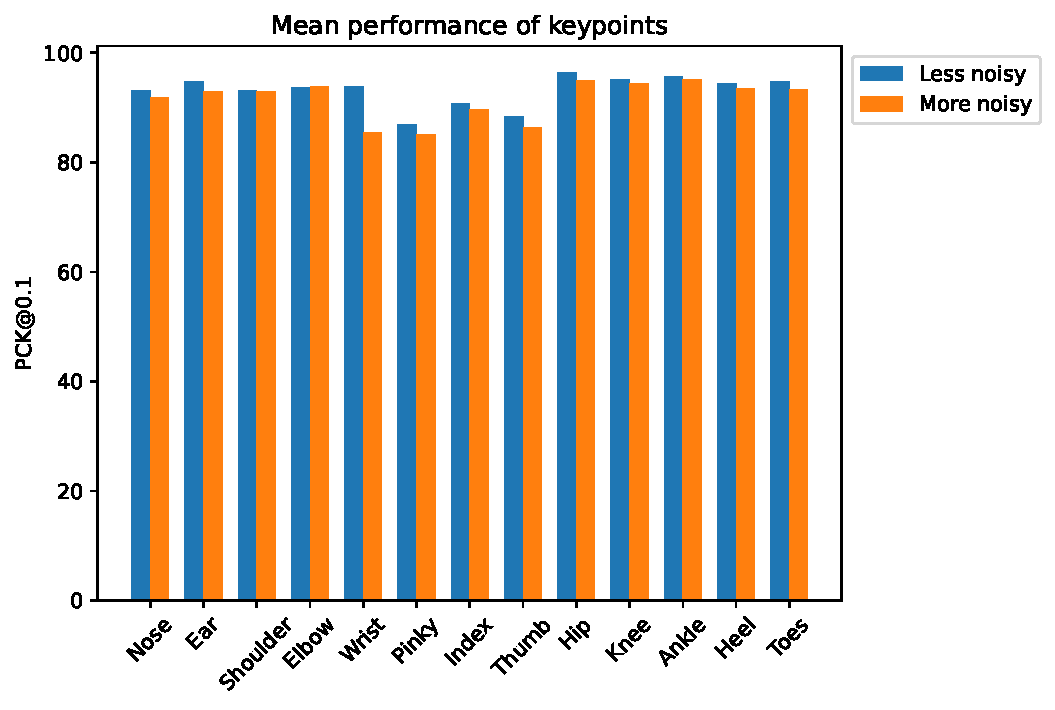
\includegraphics[width = 0.7\textwidth]{entities/kpts.pdf}
    \end{figure}
\end{frame}

\begin{frame}
    \frametitle{Discussion}
    Results:
    \begin{itemize}
        \item<1-> Translation vs translation + scaling
        \item<2-> Halfing frame rate
        \item<3-> Easiest vs most difficult joints
        \item<4-> Experiment 1 vs experiment 2
        \item<5-> Effects of pretraining
        \item<6-> Worst performing keypoints
    \end{itemize}
\end{frame}

\begin{frame}
    \frametitle{Discussion}
    All models performed better during finetuning than pretraining
    \begin{enumerate}
        \item<1-> More data
        \item<2-> Semantically different videos in pretraining
        \item<3-> Noise in BRACE annotations
        \item<4-> Frame rate in Penn Action
        \item<5-> Performace of identity function
    \end{enumerate}
\end{frame}

\begin{frame}
    \frametitle{Discussion}
    Which model is the best?
    \begin{itemize}
        \item<1-> Greatest testing accuracy: DeciWatch 1.1/1.2
        \item<2-> Greatest rough estimation: bi-ConvLSTM Model C 1.1
        \item<3-> Speed and memory: 3DConv
    \end{itemize}
\end{frame}

\begin{frame}
    \frametitle{Discussion}
    General reflections
    \begin{itemize}
        \item<1-> Pretraining
        \begin{itemize}
            \item<1-> Should have estimated parameters of data
            \item<2-> Overlapping video sequences
        \end{itemize}
        \item<3-> Finetuning
        \begin{itemize}
            \item<3-> Groundtruth outside of bbox 
        \end{itemize}
    \end{itemize}
\end{frame}

\begin{frame}
    \frametitle{Discussion}
    Future work
    \begin{enumerate}
        \item<1-> DeciWatch with all frames
        \item<2-> DeciWatch with vision transformer
        \item<3-> Avoid overfitting
        \item<4-> Multiple retraining
    \end{enumerate}
\end{frame}

\begin{frame}
    \frametitle{Conclusion}
    Succesfully developed and tested the incorporation of temporal smoothing for pose estimation
\end{frame}

\begin{frame}
    \frametitle{Extras: Mistakes Were Made!}
    Misimplemented evaluation-function
    \begin{itemize}
        \item Generally, same patterns
        \item Decreased accuracies
        \item Models do not improve the rough estimates
        \item bi-ConvLSTM: Model C is now always better than Model S
    \end{itemize}
    \begin{table}[htbp]
        \scalebox{0.7}{
            \begin{tabular}{c||ccc|ccc|ccc}
                \hline
                Accuracy metric & \multicolumn{3}{c}{PCK@0.05} & \multicolumn{3}{c}{PCK@0.1} & \multicolumn{3}{c}{PCK@0.2} \\
                \hline
                Experiment & 1.1 & 1.2 & 1.3 & 1.1 & 1.2 & 1.3 & 1.1 & 1.2 & 1.3 \\
                \hline
                \hline
                Identity function & 19.4 & 19.4 & 19.4 & 66.1 & 66.1 & 66.1 & 85.2 & 85.2 & 85.2 \\
                3DConv & 33.3 & 33.4 & 32.8 & 72.5 & 72.4 & 73.1 & 85.8 & 85.8 & 86.0 \\
                DeciWatch & 32.8 & 33.8 & 30.9 & 68.0 & 68.1 & 62.7 & 85.1 & 84.9 & 82.8 \\
                bi-ConvLSTM - Model S & 31.7 & 30.1 & 31.6 & 71.5 & 68.3 & 71.3 & 86.3 & 82.5 & 86.2 \\
                bi-ConvLSTM - Model C & 32.0 & 32.2 & 31.8 & 72.2 & 72.2 & 71.4 & 86.6 & 86.5 & 86.5 \\
                \hline
            \end{tabular}
        }
    \end{table}
    
    \begin{table}[htbp]
        \scalebox{0.7}{
            \begin{tabular}{c||ccc|ccc|ccc}
                \hline
                Accuracy metric & \multicolumn{3}{c}{PCK@0.05} & \multicolumn{3}{c}{PCK@0.1} & \multicolumn{3}{c}{PCK@0.2} \\
                \hline
                Experiment & 2.1 & 2.2 & 2.3 & 2.1 & 2.2 & 2.3 & 2.1 & 2.2 & 2.3 \\
                \hline
                \hline
                Identity function & 19.4 & 19.4 & 19.4 & 66.1 & 66.1 & 66.1 & 85.2 & 85.2 & 85.2 \\
                3DConv & 33.1 & 33.3 & 32.7 & 72.1 & 72.3 & 72.6 & 85.6 & 85.7 & 85.6 \\
                DeciWatch & 21.3 & 26.4 & 19.4 & 51.1 & 58.7 & 48.1 & 77.1 & 81.0 & 77.0 \\
                bi-ConvLSTM - Model S & 30.9 & 31.6 & 30.6 & 71.2 & 71.6 & 70.7 & 86.0 & 86.1 & 86.2 \\
                bi-ConvLSTM - Model C & 31.5 & 32.2 & 30.8 & 71.8 & 72.0 & 71.9 & 86.4 & 86.4 & 86.5 \\
                \hline
            \end{tabular}
        }
    \end{table}
\end{frame}

\end{document}